\section{Introduction}

\subsection{Overview}

A connected sum of manifolds is made by removing a disc from each manifold and gluing the manifolds along the boundary.

\begin{figure}[h]
\subfigure[Two surfaces with discs removed]{
	\label{fig:first}
	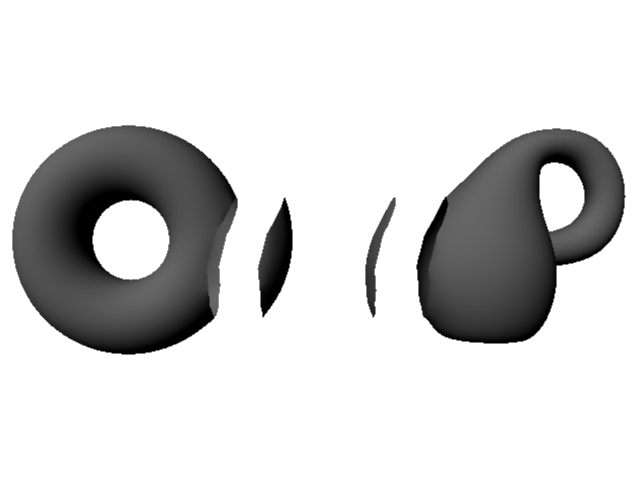
\includegraphics[scale=0.17]{../images/RemovedDiscs.png}
}
\subfigure[Two spaces naively connected]{
	\label{fig:second}
	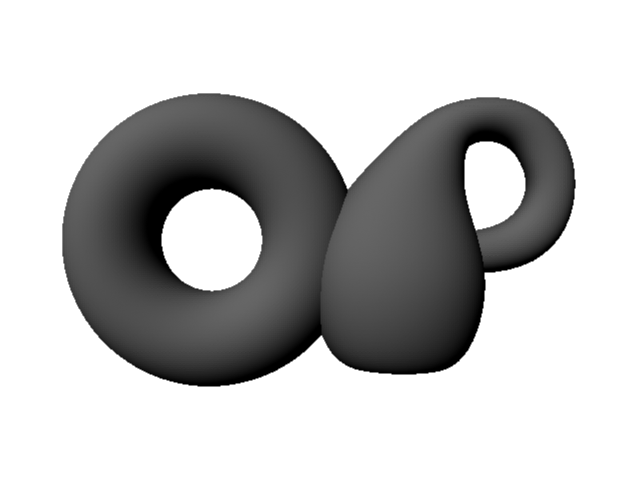
\includegraphics[scale=0.17]{../images/IntersectingSpaces.png}
}
\subfigure[Two spaces smoothly connected]{
	\label{fig:third}
	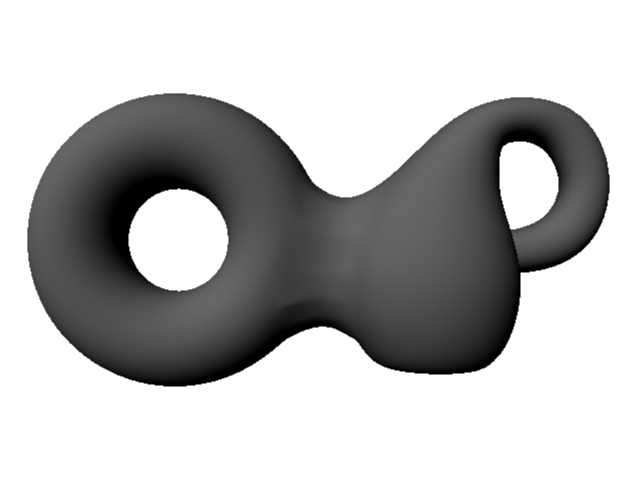
\includegraphics[scale=0.17]{../images/MergedSpaces.png}
}
\caption{Connecting two surfaces}
\end{figure}

We have written a graphics program to visualize three-dimensional non-Euclidean geometry, with emphasis on connected sums of manifolds. Our program is designed to use an intermediate manifold to allow them to be connected smoothly.

We have implemented $\mathbb{E}^3$ and a space homeomorphic to $S^2 \times \mathbb{R}$, which we have called Wormhole.

We have also implemented a method to glue multiple spaces together along spherical boundaries.

Outside Euclidean geometry, gluing spaces together like this won't always be smooth. More precisely, since two spheres with the same surface area do not generally have the same curvature, gluing the spaces together by those spheres will result in them having different curvature from each side. A similar problem will occur if the insides or outsides of two spheres are glued together.

In order to address this problem, we have designed a manifold we call the wormhole.

\begin{figure}[h]
\subfigure[Two spaces naively connected]{
	\label{fig:first}
	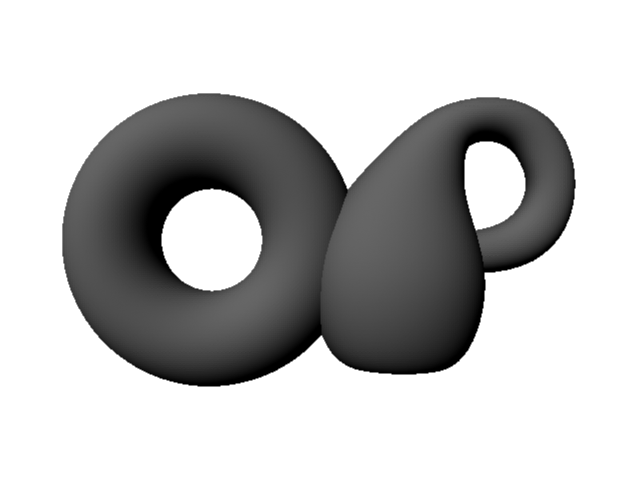
\includegraphics[scale=0.2]{../images/IntersectingSpaces.png}
}
\subfigure[A wormhole]{
	\label{fig:second}
	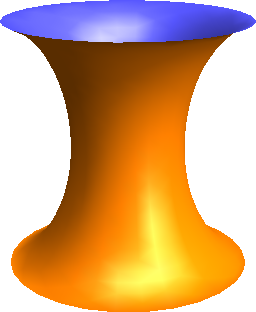
\includegraphics[scale=0.3]{../images/PortalSpace.png}
}
\subfigure[Two spaces smoothly connected]{
	\label{fig:third}
	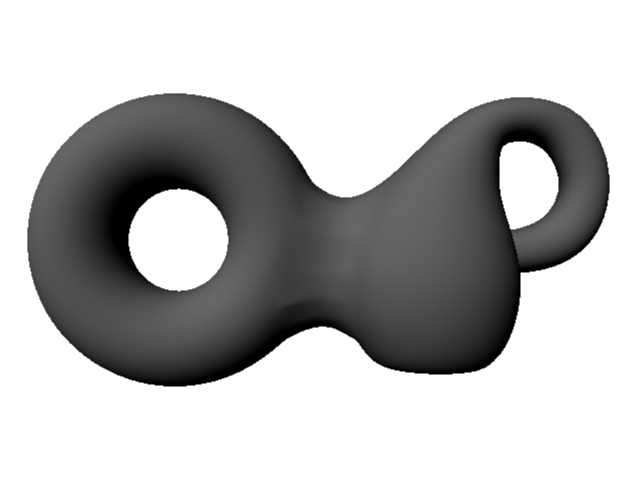
\includegraphics[scale=0.2]{../images/MergedSpaces.png}
}
\caption{}
\end{figure}

%I define an $(n,m)$-surface of revolution as an $(n+m)$-manifold which has a homeomorphism, $\phi$, to a subspace of $S^n \times \mathbb{R}^m$ which preserves??? the automorphisms that act as automorphisms on $S^n$ and preserve $\mathbb{R}^m$. An $(n,m)$-surface of revolution is also an $(n-1,m+1)$-surface of revolution for all $n \geq 1$. In addition, this definition is based entirely upon the intrinsic geometry of the space, and does not require embedding into Euclidean geometry.

%A $2$-wormhole is a $(1,1)$-surface of revolution of constant negative Gaussian curvature. This makes it a quotient space on $\mathbb{H}^2$, for which it is easy to find geodesics.

We define $2$-Wormhole as a quotient space on $\mathbb{H}^2$ made by identifying two ultraparallel lines. We have designed $3$-Wormhole as a higher-dimensional analogue of a $2$-wormhole. %This is a $(1,1)$-surface of revolution.

\ignore{
An $n$-wormhole is an $(n-1,1)$-surface of revolution. Generally, this does not have constant curvature, and is not a quotient space on $\mathbb{H}^n$. However, we have found a method to reduce finding a geodesic on an $(n,m)$-surface of revolution to a $(1,m)$-surface of revolution. In particular, I can find the geodesic on an $n$-wormhole using the method to find a geodesic on a $2$-wormhole.

There are two other spaces that are similar to this wormhole that are of interest. We hope to program these, but they are not part of my main goal. If I run out of time, I will consider the project complete without them. I call one a black hole and the other a cone point space. These spaces, and the wormhole, all are built by extending to the third dimension a quotient space of $\mathbb{H}^2$ in which two lines are identified. The wormhole occurs if the two lines are ultraparallel, the black hole if they're asymptotic, and the cone point space if they intersect.

Black holes and cone spaces can support the connection of two spaces in a similar manner, but they're more interesting just connected to one. \ignore{Why?} An $n$-black hole is an $n$-dimensional analogue of a pseudosphere, in which the embedding into $\mathbb{E}^3$ which has spherical cross-sections instead of circular ones. An $n$-cone point space is notable for containing a cone point and still being easy to connect to $\mathbb{E}^n$ or $\mathbb{H}^n$.

Another way to generalize this is to identify lines on $\mathbb{E}^2$ or $S^2$ instead of $\mathbb{H}^2$. Again, this is not part of the main project, and is not required for me to consider it complete.

Identifying two parallel lines on $\mathbb{E}^2$ creates a cylinder, which extends to $\mathbb{S}^n \times \mathbb{R}$. Identifying two intersecting lines creates a cone, which extends to a higher dimensional cone. Identifying two lines on a sphere creates something shaped like a lemon, with two cone points on opposite sides. If you extend this to identify two lines that meet at an angle greater than $360^\circ$, which you can construct by gluing multiple spheres together, the resulting space cannot be embedded in $\mathbb{E}^3$.

This variation is particularly interesting because it contains a cone point of angle greater than $360^\circ$ and can be smoothly attached to $\mathbb{E}^n$ and $S^n$. While these cone points can be made easily by generalizing the Cone Point Space and hypercones, they can be smoothly attached only to $\textbf{H}^3$ and $(n-1,1)$-surfaces of revolution. Furthermore, the only $(n-1,1)$-surface of revolution that I have defined that could be used as an intermediate manifold to attach a Cone Point Space or hypercone to $\textbf{E}^n$ or $S^n$ is this manifold. In addition, this variation can be used as an intermediate space to glue a ball of $\textbf{H}^n$ into $\textbf{E}^n$ or $S^n$, producing an area that is smaller on the inside.

Figures 1-4 illustrate the $2$-dimensional versions of these surfaces. While only the portion of the surfaces that can be embedded into $\mathbb{E}^3$ are shown here, my program will be capable of presenting the entire surface for visualization.

\begin{figure}[h]
\subfigure[Part of a 2-wormhole]{
	\label{fig:first}
	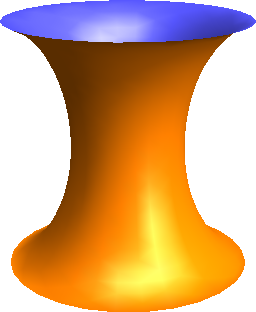
\includegraphics[scale=0.33333]{../images/PortalSpace.png}
}
\subfigure[Part of a 2-black hole space]{
	\label{fig:second}
	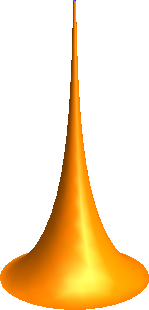
\includegraphics[scale=0.33333]{../images/BlackHole.png}
}
\subfigure[Part of a 2-cone point space]{
	\label{fig:third}
	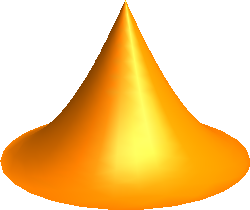
\includegraphics[scale=0.33333]{../images/ConePoint.png}
}
\subfigure[Part of a 2-extended sphere]{
	\label{fig:fourth}
	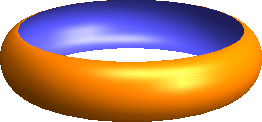
\includegraphics[scale=0.33333]{../images/OuterTorus.png}
}
\end{figure}

I also hope to implement $S^3$ and $S^2 \times \mathbb{R}$. I may also implement $\mathbb{H}^2 \times \mathbb{E}$, but it doesn't combine well with the wormhole, so it won't be as useful.
}

One obstacle was finding geodesics between two given points when spaces are glued together. Since light follows a geodesic, this is necessary to show where you'd see the point. In $E^3$ and Wormhole, it is not difficult to construct a geodesic between two given points. However, this does not apply to their connected sums.

I can easily construct a geodesic from a given point moving in a given direction. By repeatedly constructing such geodesics at set lengths and taking note of the error, I can use Newton's method to solve numerically for the geodesic between two given points.

My program can be run either through rasterization or ray-tracing.

When used for rasterization, the program finds a geodesic from the camera to each vertex, finds the direction the geodesic moves from the camera, and draws the vertex in that direction. Then it draws triangles between those vertices.

When used for ray-tracing, it constructs geodesics corresponding to each pixel in the camera, and shoots rays to see what lies in that direction. \ignore{This leads to problems with light sources, since I still need to find the angle and distance of the light source from the given point. I have found three possible solution:

\begin{itemize}

\item We can give every point the same lighting, regardless of position. This will likely be useful for debugging, but it results in no shading, which will make it less useful or interesting.

\item We can use the camera as the light source. In this case, the geodesic that passes between the camera and a given point is the one We used to find that point to begin with. The shading will be a function only of distance, unless Phong shading is used. It will look better, but it will still be very limited.

\item We can simple fire photons in various directions from the light sources, and use them to color objects they strike. Photons can be used to give effects that are otherwise impossible, such as diffuse interreflection, where an object is illuminated by light reflected off of another object, but they generally take a very long time to calculate.

\end{itemize}

There is another notable detail. In Euclidean geometry, lighting falls of inversely with the square of distance. This does not apply in general. Changing the direction and distance a photon is emitted by $\varepsilon\textbf{u}$ for some unit vector $\textbf{u}$ will change where it hits by $M\varepsilon\textbf{u} + O(\varepsilon^2)$ for some matrix $M$. The brightness is inversely proportional to $|\det(M)|$.

More accurately, given the list of all vectors $\textbf{v}_1, \textbf{v}_2, ...$ such that the photons moving in that direction for that distance hit the given point, the brightness at that point is proportional to $\sum\frac{1}{|\det(M_{\textbf{v}_i})|}$. This is because, in general, two points can be connected by more than one geodesic.
}

\ignore{1.  Describe 3-manifold decompositions.
  A.  Prime decomposition theorem -- see Allen Hatcher's notes for statement and references.

%http://www.math.cornell.edu/~hatcher/3M/3M.pdf
}
\ignore{@Misc{•,
OPTkey = {•},
OPTauthor = {Allen Hatcher},
OPTtitle = {Notes on Basic 3-Manifold Topology},
OPThowpublished = {•},
OPTmonth = {•},
OPTyear = {•},
OPTnote = {•},
OPTannote = {•}
}}

\subsection{Background}

The prime decomposition theorem states that a compact, connected, orientable 3-manifold can be decomposed into a connected sum of prime manifolds (manifolds that cannot be decomposed further, except by trivially removing a sphere) \cite{Kneser}, and that this is unique up to insertion or deletion of copies of $S^3$ \cite{Milnor}. The connected sum of two spaces is made by removing a ball from each and identifying their bounding spheres.
%What are the prime manifolds? What about manifolds that are not compact or are not orientable?
  
%  B.  Torus decomposition theorem -- see Allen Hatcher's notes for statement and references.

The torus decomposition theorem states that there is a minimal collection of disjointly embedded incompressible tori such that cutting along each yields components that are each either atoroidal or Seifert-fibered. It also states that this collection is unique up to isomorphism \cite{JSJ3} \cite{JSJ2} \cite{JSJ1} \cite{JSJ4}.

%Wikipedia has four references. Which do I use?

%  C.  Geometrization theorem.  (Wikipedia probably has statement, references?)

The geometrization theorem states that any 3-manifold can be decomposed canonically into submanifolds which each is a quotient space of one of the following eight geometries: $S^3, \mathbb{E}^3, \mathbb{H}^3, S^2 \times \mathbb{R}, \mathbb{H}^2 \times \mathbb{R}, \tilde{SL}(2,\mathbb{R}),$ Nil geometry, and Sol geometry. This is done by decomposing along the spheres given by the prime decomposition theorem and tori given by the torus decomposition theorem. The initial work was done by Grisha Perelman \cite{Perelman1} \cite{Perelman3} \cite{Perelman2}, and was later completed by other mathematicians \cite{Geometrization1} \cite{Geometrization2} \cite{Geometrization3}.

%  [D.  Your work:  take some of 8 geometries, glue together via "smooth" prime decomposition.]

My program allows the smooth creation of a connected sum of Euclidean geometries as in the geometrization theorem, and visualization of the result. My program can also be easily expanded to include hyperbolic and spherical geometry. ``Smoothness'' means that the boundaries that are identified have the same curvatures in each surface. If they are not smoothly identified, then they will appear to have different curvatures from each side. As a result, a geodesic that barely intersects the border can have a very different path from one that barely misses.

For example, if we glue the outside of a sphere in Euclidean geometry to the outside of another such sphere in another copy of Euclidean geometry, the result looks like the portal is a reflective sphere, but with the reflection from the other geometry. This has effects such as blocking anything behind the sphere. This is impossible in a true manifold. Any point is visible from any other. My program avoids this by using an intermediate geometry of non-constant curvature which contains spheres that can be glued to spaces of any constant curvature.

My program does not support torus decompositions, and cannot show every manifold. However, it is still more general than anything that has been reported previously, as described next.

%Additionally, I hope to make my program run real-time. While this is common for programs simulating spherical, Euclidean, and hyperbolic geometry, I do not believe it has been done for more sophisticated geometries, as there is not enough time to find geodesics numerically.

%Cone points?

%I also hope to add cone points to my program.


%2.  Visualizing 3-manifolds.
%  A.  Jeff Weeks website -- compact manifolds of constant curvature

Previous work has been done to visualize $S^3$ and $\mathbb{H}^3$ and quotient spaces thereof. In particular, Weeks has written a program that can view compact quotient spaces of $S^3, \mathbb{E}^3,$ and $\mathbb{H}^3$ \cite{CurvedSpaces}. He also wrote a paper that describes the process in depth \cite{CurvedSpacesPaper}.

Gunn and Maxwell made a video showing the complementary spaces of knots, most of which are quotient spaces of $\mathbb{H}^3$ \cite{NotKnot}. Gunn explains the techniques he uses in \cite{CharlieGunn} \cite{CharlieGunn2}.

Levy, Munzner and Mark Phillips wrote a geometry viewer called Geomview. Among its features is the ability to render non-Euclidean geometry \cite{Geomview}.

The main difference that distinguishes my work is the ability to create connected sums between spaces.

%  B.  Youtube movie

%http://www.spacetimetravel.org/wurmlochflug/wurmlochflug.html

We are unaware of any previous attempts to visualize general connected sums of geometries. However, attempts have been made to visualize a connected sum of two $\mathbb{E}^3$ spaces, with curvature near zero outside of a small wormhole.

Rune Johansen made a video that was designed to convey the idea of a wormhole \cite{runevision}. This video is primarily artistic in nature, and uses various tricks to make space look curved. There is no geometry that looks precisely like the video.

Corvin Zahn made a computer generated video precisely illustrating a wormhole \cite{spacetimetravel}. He uses a solution to Einstein's field equations that had been found previously \cite{WormholeSolution}, and simulated the camera moving through this wormhole.

Zahn's wormhole was made as one continuous geometry with everywhere negative curvature. While this is a much more interesting space than what my program will make, it's much harder to generalize. Adding a second wormhole between the spaces or a second wormhole leading to a third space would require redesigning the entire manifold. In contrast, my program provides a compact manifold with boundary to connect spaces, so as long as the spheres they replace in Euclidean geometry do not touch, any number can be added easily to the same space.

In adddition, Zahn seems to have used a ray-tracing method and found the geodesics numerically. My program can use rasterization to run at near real-time, or solve geodesics symbolically to speed up ray-tracing.

%  C.  Other?  E.g. old references on visualizing hyperbolic geometry?

%3.  Cone manifolds
%  A.  Define.  For example see definition in book "Three-dimensional orbifolds and cone manifolds" by Cooper, Hodgson, Kerckhoff.  Find other references there.
%  [B.  Note they are typically studied for manifolds of constant sectional curvature.  You will look at nonconstant.]

%Is this the same as the Sasakian manifold?

%https://en.wikipedia.org/wiki/Clairaut's_relation Good for solving surfaces of revolution numerically.